\begin{center}\small
\begin{tabularx}{\linewidth}{@{}l>{\raggedleft\arraybackslash}X>{\raggedleft\arraybackslash}X>{\raggedleft\arraybackslash}X@{}}
\toprule
Pair & Gaussian $K$ range & Block $K$ range & Swaps G/B\\
\midrule
P1 & [0.737, 0.757] & [0.737, 0.753] & 8/3\\
P2 & [0.691, 0.733] & [0.698, 0.728] & 21/10\\
P3 & [0.707, 0.736] & [0.711, 0.737] & 1/1\\
P4 & [0.718, 0.738] & [0.721, 0.739] & 1/2\\
P5 & [0.661, 0.705] & [0.661, 0.707] & 0/0\\
P6 & [0.686, 0.702] & [0.688, 0.702] & 0/0\\
\bottomrule
\end{tabularx}
\end{center}
G/B counts use 400 draws per method. They are bootstrap selection frequencies under the working mechanism, not posterior probabilities of a physical pole assignment.
\begin{center}\small
\begin{tabularx}{\linewidth}{@{}l>{\raggedleft\arraybackslash}X>{\raggedleft\arraybackslash}X@{}}
\toprule
Pair & Unlabeled slow pole, s & Unlabeled fast pole, s\\
\midrule
P1 & [146.1, 150.7] & [16.1, 17.1]\\
P2 & [117.5, 138.7] & [19.6, 24.6]\\
P3 & [132.8, 140.6] & [17.9, 19.0]\\
P4 & [144.9, 150.4] & [15.5, 16.7]\\
P5 & [127.6, 131.8] & [18.3, 20.9]\\
P6 & [129.3, 132.0] & [18.3, 19.3]\\
\bottomrule
\end{tabularx}
\end{center}
These are Gaussian percentile ranges. Unlabeled poles avoid combining two swapped parameter basins in a single interval for a physical time constant.
\begin{center}\small
\begin{tabularx}{\linewidth}{@{}l>{\raggedleft\arraybackslash}X>{\raggedleft\arraybackslash}X>{\raggedleft\arraybackslash}X@{}}
\toprule
Pair & $K$ width: 30-s blocks & 60-s blocks & 120-s blocks\\
\midrule
P1 & 0.0147 & 0.0152 & 0.0163\\
P2 & 0.0293 & 0.0298 & 0.0481\\
P3 & 0.0257 & 0.0265 & 0.0215\\
P4 & 0.0215 & 0.0183 & 0.0180\\
P5 & 0.0447 & 0.0455 & 0.0460\\
P6 & 0.0148 & 0.0141 & 0.0127\\
\bottomrule
\end{tabularx}
\end{center}
Widths are in $\C/\%$. Blocks count samples, approximately seconds. The 30/120-s sensitivities use 100 draws each; their 2.5\% tails involve only two or three order statistics. The 400-draw primary methods have about ten draws per tail. Rare pole switches can move endpoints; the archive retains order-statistic Monte Carlo ranges and half-batch discrepancies.
\begin{center}\small
\begin{tabularx}{\linewidth}{@{}l>{\raggedleft\arraybackslash}X>{\raggedleft\arraybackslash}X>{\raggedleft\arraybackslash}X@{}}
\toprule
Pair & Smallest information eigenvalue & Condition & Weak log direction\\
\midrule
P1 & 2.77e+03 & 43.8 & (-0.26, -0.36, 0.89)\\
P2 & 191 & 10.5 & (0.13, -0.49, 0.86)\\
P3 & 2.04e+03 & 22.3 & (0.54, 0.72, -0.44)\\
P4 & 1.5e+03 & 53.8 & (-0.33, -0.42, 0.84)\\
P5 & 791 & 62.1 & (-0.46, -0.11, 0.88)\\
P6 & 5.28e+03 & 15.5 & (0.26, -0.24, 0.94)\\
\bottomrule
\end{tabularx}
\end{center}
Directions use $(\log K,\log\tau,\log\theta)$ after eliminating ambient columns; eigenvector signs are arbitrary. These are local fixed-covariance diagnostics and ignore box geometry and separated modes.
All six conditional thermal information matrices have rank three at relative eigenvalue thresholds $10^{-8}$, $10^{-10}$ and $10^{-12}$. P2's full observed curvature is indefinite, so its regular Gaussian covariance is withheld. P4 has an active ambient bound despite positive observed curvature. Rank and positive curvature alone do not settle bounded or global inference.
\begin{center}\small
\begin{tabularx}{\linewidth}{@{}l>{\raggedleft\arraybackslash}X>{\raggedleft\arraybackslash}X>{\raggedleft\arraybackslash}X>{\raggedleft\arraybackslash}X@{}}
\toprule
Pair & OLS RMSE & GLS RMSE & Common sines & Ambient reconstruction\\
\midrule
P1 & 2.175 & 2.219 & 2.168 & 0.930\\
P2 & 1.605 & 1.695 & 1.736 & 0.606\\
P3 & 2.038 & 1.950 & 1.831 & 0.629\\
P4 & 1.881 & 1.881 & 1.625 & 0.576\\
P5 & 1.853 & 2.223 & 1.431 & 1.085\\
P6 & 1.856 & 1.856 & 1.358 & 0.684\\
\bottomrule
\end{tabularx}
\end{center}
RMSE is in degrees Celsius. OLS/GLS columns pool each pair's ten evaluation records; the exclusions differ, so those aggregates are not a controlled same-test-set ranking. Common sines restrict GLS evaluation to 30-s run 1, 120-s run 3 and 300-s run 2, which are excluded from all six calibrations. Primary predictions use zero future ambient correction. The last column fits an offset using the complete evaluation response and is retrospective reconstruction.
\begin{center}\small
\begin{tabularx}{\linewidth}{@{}l>{\raggedleft\arraybackslash}X>{\raggedleft\arraybackslash}X>{\raggedleft\arraybackslash}X@{}}
\toprule
Pair & Gaussian inside, \% & Block inside, \% & Gaussian + ambient, \%\\
\midrule
P1 & 19.0 & 20.5 & 58.5\\
P2 & 55.3 & 43.6 & 100.0\\
P3 & 32.9 & 29.3 & 89.8\\
P4 & 16.8 & 20.0 & 73.1\\
P5 & 50.8 & 54.2 & 80.7\\
P6 & 15.7 & 14.8 & 79.0\\
\bottomrule
\end{tabularx}
\end{center}
Fractions count measured temperatures inside pointwise future-observation ranges, pooled by sample count. Ambient envelopes are scenarios. Overlapping evaluation records and serial dependence prevent independent-binomial coverage claims.
\begin{figure}[htbp]\centering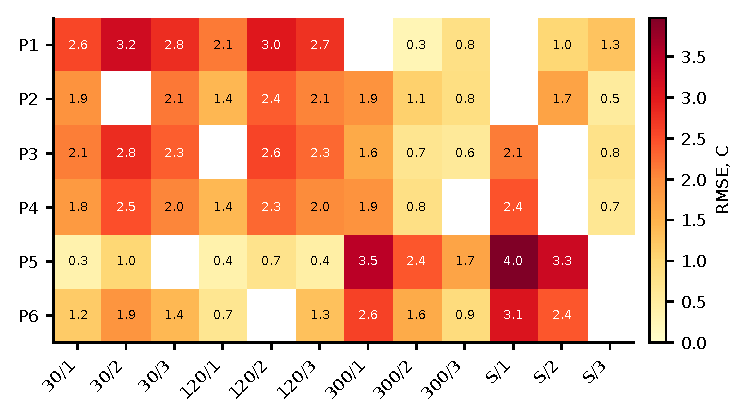
\includegraphics[width=\linewidth]{generated/figures/prediction_RMSE.pdf}\caption{Zero-ambient prediction RMSE in degrees Celsius. White cells are the two calibration records for that pair. Records are labeled by sine period or step (S), then run number.}\end{figure}
